
\begin{frame}
  \frametitle{SPICE Open Source Clones: Many initiatives \ldots !}
  \begin{enumerate}
  \item \textbf{Berkeley spice3f5} \alert{1996}
    \begin{itemize}
    \item A Research Project
    \item Source code \alert{was not developed with industrial Q\&A}
    \end{itemize}
  \item \textbf{Ngspice} (New Generation Spice)
    \begin{itemize}
    \item \alert{Fork of Berkeley spice3f5}
    \item Features mixed-level and mixed-signal simulation \\
      XSpice (mixed signal), Cider1b1 and GENIUS TCAD (mixed level)
    \item \alert{Still maintained (?) but not actively !}
      % \item Manual has 600 pages
    \end{itemize}
  \item \textbf{GnuCap} (GNU Circuit Analysis Package)
    \begin{itemize}
    \item Attempt to rewrite SPICE from scratch by Albert Davis in \alert{1993}
    \item Davis's Thesis "Implicit Mixed-Mode Simulation of VLSI Circuits"
    \item No longer maintained since 2006 (2013 ?)
    \end{itemize}
  \item \textbf{QUCS} (Quite Universal Circuit Simulator) \alert{2003}
  \item \textbf{Akhab} \alert{2006}
  \end{enumerate}
\end{frame}

\begin{frame}
  \frametitle{QUCS: When Open Source fails !}
  \begin{columns}
    \begin{column}{.6\textwidth}
      \centerline{QUCS: Quite Universal Circuit Simulator}
      \begin{itemize}
      \item Founded by Michael Margraf in 2003 (?)
      \item \textbf{IDE} based on Qt3 \\
      \item \textbf{Complete Toolchain} \\
        Schematic Editor, Simulation and Plot
      \item \textbf{Interesting simulation features}
      \item Margraf moved later to proprietary software ???
      \item Slowly maintained \\
        port to Qt4 is ongoing since \ldots many years
      \end{itemize}
    \end{column}
    \begin{column}{.4\textwidth}
      \begin{center}
        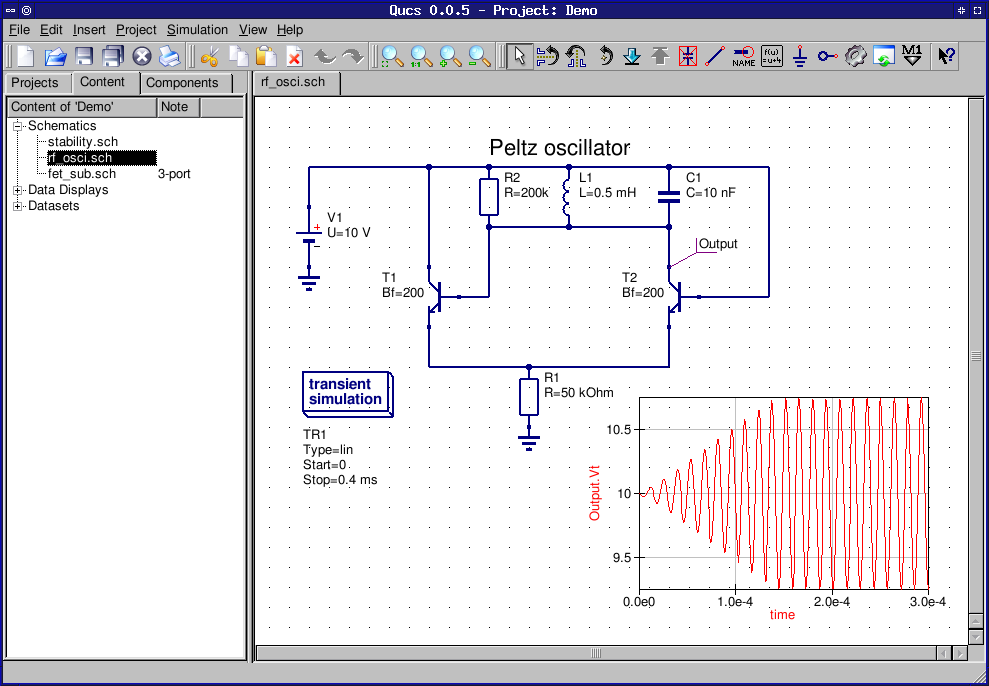
\includegraphics[width=1.\textwidth]{images/qucs.png}
      \end{center}
    \end{column}
  \end{columns}
\end{frame}

\begin{frame}
  \frametitle{QUCS: What is wrong ?}
  \begin{columns}
    \begin{column}[t]{.5\textwidth}
      To develop an electric CAD software, \\
      we need these \textbf{skills} and \textbf{budgets}
      {\footnotesize
        \begin{itemize}
        \item Circuit Simulation
        \item Solid State Device Modelling
        \item State of Art Numerical Analysis
        \item Software Architecture, Core Design
        \item GUI Design
        \item XML Format Design
        \item Schematic Editor Design
        \item Plot Library
        \item \ldots
        \end{itemize}%
      }
      \begin{textblock}{6}(4,6.5)
        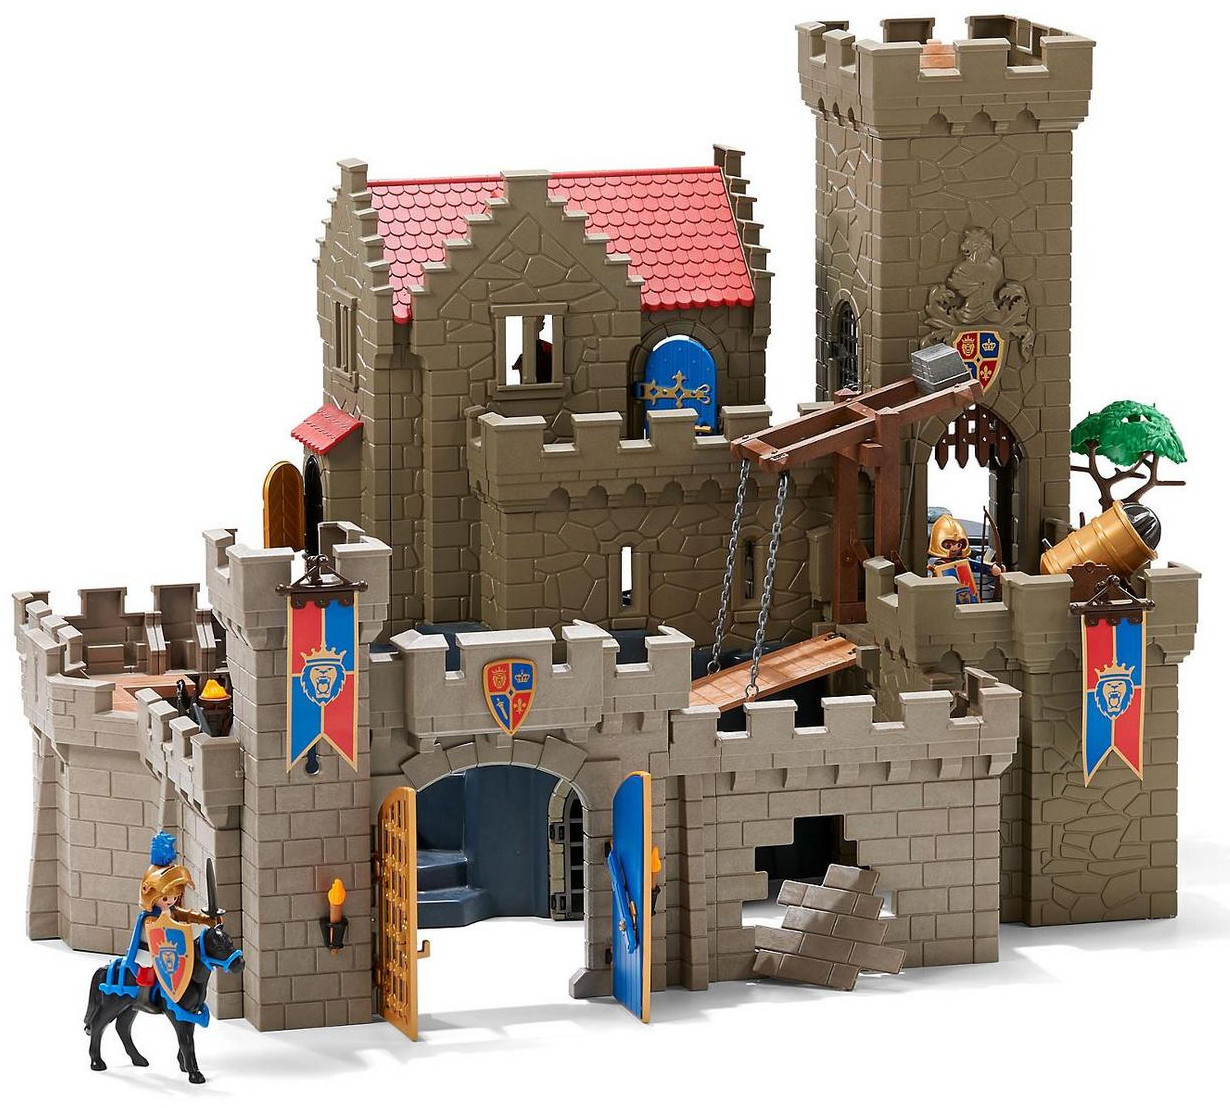
\includegraphics[width=.4\textwidth]{images/playmobil.jpg}
      \end{textblock}
    \end{column}
    \begin{column}[t]{.5\textwidth}
      Later, We have to \alert{maintain} \\[.5em]
      \begin{itemize}
        \item A very large code base
        \item A GUI Qt3 $\rightarrow$ Qt4 $\rightarrow$ Qt5 $\rightarrow$ \ldots \\[1em]
      \end{itemize}
      \alert{Don't do that} until you have a zillion \$ (industrial market) \\[1em]
      \alert{\textbf{Develop Software Components !}} \\
      \alert{\textbf{And plug them together}} \\
      
\includegraphics[width=.5\textwidth]{images/lego2.jpg}
    \end{column}
  \end{columns}
\end{frame}

%%% Local Variables:
%%% mode: latex
%%% TeX-master: "master"
%%% End:
